\chapter{Sand extraction}
\section{Dredging activities}
This section describes the relevance of dredging to the sediment balance of the designated area, by an estimation of the dredging volumes, through AIS data and extraction permits.

\subsection{Vessel positioning information (AIS)}
Using MarineTraffic it was found that two dredgers are operating on the Paraná Guazú between Ibicuy and Brazo Largo: the Comercio Segundo and the E.M. Arroyo N1. The Comercio Segundo has a length of 30 m, a width of 7 m, a draft of 1.3 m, and an approximate cargo hold of 195 m\textsuperscript{3}. The E.M. Arroyo N1 has a length of 39 m, a width of 8 m, a draught of 2.8 m and an approximate cargo hold of 476 \,m\textsuperscript{3}. Using a sand to water ratio of 3:1 for the dredged slurry, the amount of sand dredged is 150 \,m\textsuperscript{3} and 360 \,m\textsuperscript{3} respectively per cargo. The tracks of the two vessels obtained from MarineTraffic are shown in Figures 5.1 and 5.2.

\begin{figure}[H]
    \centering
    \begin{minipage}{0.48\textwidth}
        \centering
        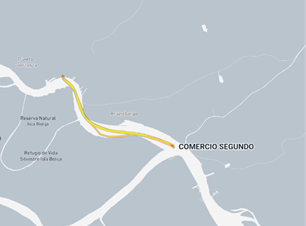
\includegraphics[width=\linewidth]{figures/ch5/Track_CS.png}
        \caption{Track of the \textit{Comercio Segundo}}
        \label{fig:track_cs}
    \end{minipage}\hfill
    \begin{minipage}{0.48\textwidth}
        \centering
        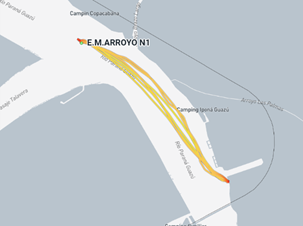
\includegraphics[width=\linewidth]{figures/ch5/Track_EM.png}
        \caption{Track of the \textit{E.M. Arroyo N1}}
        \label{fig:track_em}
    \end{minipage}
\end{figure}

The AIS data for these two vessels is obtained from MyShipTracking, which is used to determine the location of the dredging and the average number of trips. The dredging location of the two vessels is shown in Figure 5.3. It can be seen that both dredgers dredge in the same area. This can be explained by the bathymetry shown in Figure 5.4, which shows a reduced depth near the junction of the two navigable channels. At this location the flow velocity is lower, causing sediment to settle and thus creating a sandbar. From the AIS data it can be concluded that both dredgers make three trips per day.

\begin{figure}[H]
    \centering
    \begin{minipage}{0.48\textwidth}
        \centering
        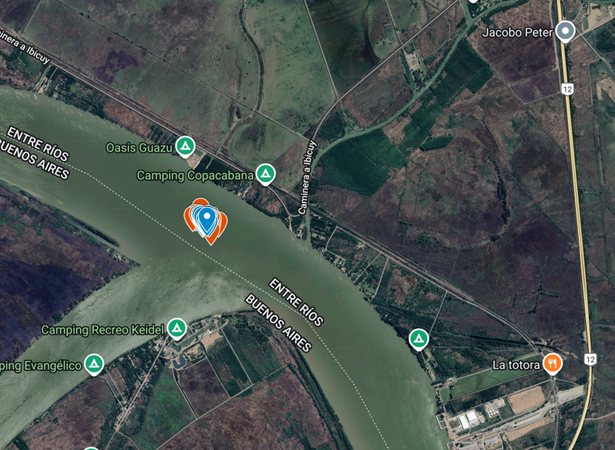
\includegraphics[width=\linewidth]{figures/ch5/Dredging_coordinates.png}
        \caption{Dredging location}
        \label{fig:dredging_coordinates}
    \end{minipage}\hfill
    \begin{minipage}{0.48\textwidth}
        \centering
        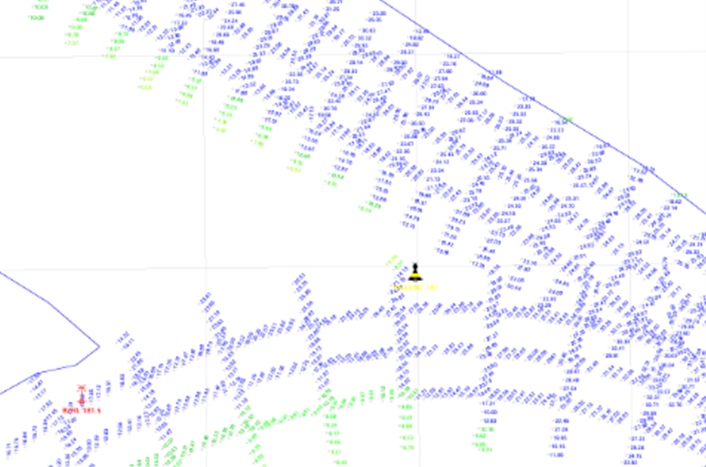
\includegraphics[width=\linewidth]{figures/ch5/Bathymetry.png}
        \caption{Bathymetry}
        \label{fig:bathymetry}
    \end{minipage}
\end{figure}

In the Rio Talabera, a side branch connecting to the Paraná Guazú, a third dredger is extracting sand. The Altair is dredger with a length of 66 m, a width of 11 m, a draught of 1.5 m and a approximate cargo hold of 750 \,m\textsuperscript{3}. Using the same sand to water ratio of 3:1 this gives 560 \,m\textsuperscript{3} of sand per cargo. Using MarineTraffic it was found that the Altair has an average 3 trips per day. Figure 5.5 shows the track of the Altair and the location at which it stops to extract sand. 

\begin{figure}[H]
    \centering
    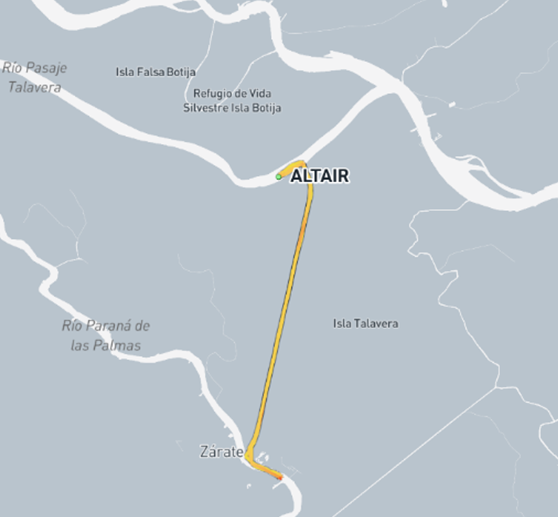
\includegraphics[width=0.5\linewidth]{figures/ch5/Track_Altair.png}
    \caption{Track of the Altair}
    \label{fig:placeholder}
\end{figure}

For all three vessels, the estimated volume of sand extracted per month is displayed in table 5.1
\begin{table}[h!]
\centering
\begin{tabular}{lrrrr}
\hline
\textbf{Vessel} & \textbf{Cargo hold} & \textbf{Sand volume [\,m\textsuperscript{3}]} & \textbf{Trips per day} & \textbf{Volume per month [\,m\textsuperscript{3}]} \\
\hline
Comercio Segundo & 195 & 150 & 3 & 9000 \\
E.M. Arroyo N1 & 476 & 360 & 3 & 21600 \\
Altair & 750 & 560 & 3 & 33600 \\
\hline
\end{tabular}
\caption{Sand transport details per vessel.}
\label{tab:sand_volume}
\end{table}

\subsection{Extraction permits}
A total of 33 permits were collected for the Paraná Guazú and 43 for the Ibicuy. On the Paraná Guazú, four permits were issued for channel maintenance, while the remainder concerned sand extraction. For the Ibicuy, all permits were related to extraction activities. The analysis shows that the requested volumes in the Ibicuy are considerably larger than those in the Paraná Guazú, even though the section of the Ibicuy considered here is much shorter in length.

It is important to note that the end dates of contracts are unknown. While the requests specify monthly dredging quantities, they do not indicate the duration of the works. As a result, a detailed quantitative assessment cannot be made. For the present analysis, all requests with fixed monthly volumes are assumed to extend over 12 months, allowing for a comparison between the two river sections, as shown in Figure \ref{fig:yearly dredging volumes}. The second assumption is to record a single value for the requested volume, when information about monthly or yearly occurrence is lacking.

\begin{figure}[H]
    \centering
    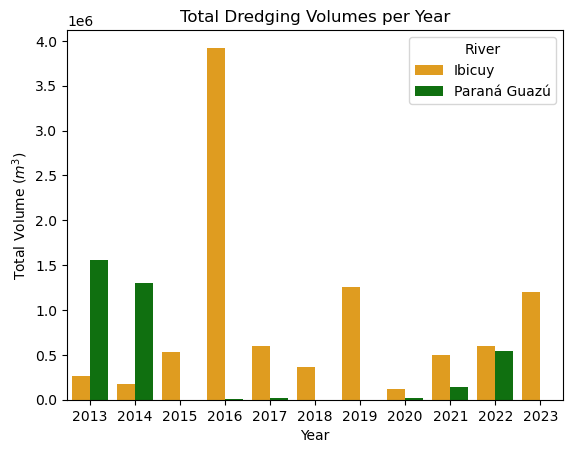
\includegraphics[width=0.50\linewidth]{figures/ch2/Dredging volumes permits.png}
    \caption{Yearly dredging volumes}
    \label{fig:yearly dredging volumes}
\end{figure}

\subsection{Estimated sand extraction}
This section draws a conclusion on the sand extraction volumes, such that an estimate is found to apply in the sediment balance. The following uncertainties were considered in determining a representative value:

\begin{itemize}
    \item Not every vessel in the area is equipped with an AIS transponder, meaning that possibly not all active vessels were identified. However, the number of vessels as found by analysis of the AIS data was in agreement with the number of vessels as observed during the fieldwork.
    \item No historical AIS data was available, such that the data was registered for only a short period of time.
    \item The extraction permits do not mention the duration of the contract.
\end{itemize}

However, a rough estimate can be found by calculating the mean annual volume for the total system of interest (i.e., Ibicuy and Paraná Guazú). To make a comparison with the monthly values in Table \ref{tab:sand_volume}, this yearly value is reduced to a monthly value by dividing by 12 months. The former approach yields the following value for dredged sand volumes:

\begin{equation}
    V_{sand,yearly} = 1193923 ~m^3
\end{equation}
\begin{equation}
    V_{sand,monthly} = \frac{V_{sand,yearly}}{12} \approx 100000 ~m^3 
\end{equation}

\section{Dry sand mining}
As mentioned in chapter \ref{chapter:stakeholders}, many stakeholders stressed the relevance of dry sand mining related to fracking for the lower delta region. In this section, context to these claims is given. The history and development of fracking in Argentina is given, followed by the geological properties of the area and the characteristics of dry sand used in fracking. Finally, the effects of dry sand mining are discussed.

\subsection{Fracking in Argentina}
For much of its history, Argentina was regarded as a modest oil producer, struggling to meet its own energy demands. This perception shifted with the 2011 discovery of the Vaca Muerta shale formation, located in the Neuquén basin in Patagonia. The Argentine energy company YPF identified approximately 150 million barrels of recoverable oil in the field, which was regarded as a new source of hope for economic stability by the president \autocite{kraussArgentinaHopesBig2011}.

The discovery was followed by significant foreign investment from companies such as Total, ExxonMobil, Apache, and EOG Resources. More exploration was done and now it is clear that Argentina possesses the world’s fourth-largest shale oil and second-largest shale gas reserves. The Government of Argentina still views the oil and gas sector as a crucial part of its economy, by driving exports as well as generating foreign currency \autocite{internationaltradeadministrationArgentinaCountryCommercial2025}.

The Nuequén basin is located in the provinces of Neuquén, Mendoza, and Río Negro in the South of Argentina and has been an important basin for oil and gas since more than a century. Production started in 1918 and in 2004, 45\% of Argentinian oil production and 61\% of its gas production came from this area \autocite{u.s.energyinformationadministrationTechnicallyRecoverableShale2013}. This was done through conventional methods, but after the discovery of the Vaca Muerta shale basin, fracking has become increasingly important for the region and the country. The Vaca Muerta shale consists of finely-stratified black to dark grey shale and lithographic lime-mudstone and is 60 to 520 m thick. Estimates are that the formation contains 16 billion barrels of technically recoverable oil and 8722 billion cubic metres of technically recoverable gas \autocite{u.s.energyinformationadministrationTechnicallyRecoverableShale2013}. Since Vaca Muerta is a shale reservoir, all oil and gas from this deposit is extracted by fracking.

As can be seen in figure \ref{fig:oilgasprod}, oil production in Argentina has been steadily increasing since 2020, driven by increased production of the Vaca Muerta formations. After the exploration in 2010, oil from Vaca Muerto as a share of total Argentinian oil production has increased from virtually 0\% to 55\% today. Further, Vaca Muerta now accounts for 47\% of gas supply (PPT) \autocite{internationaltradeadministrationArgentinaCountryCommercial2025}.

\begin{figure}[H]
    \centering
    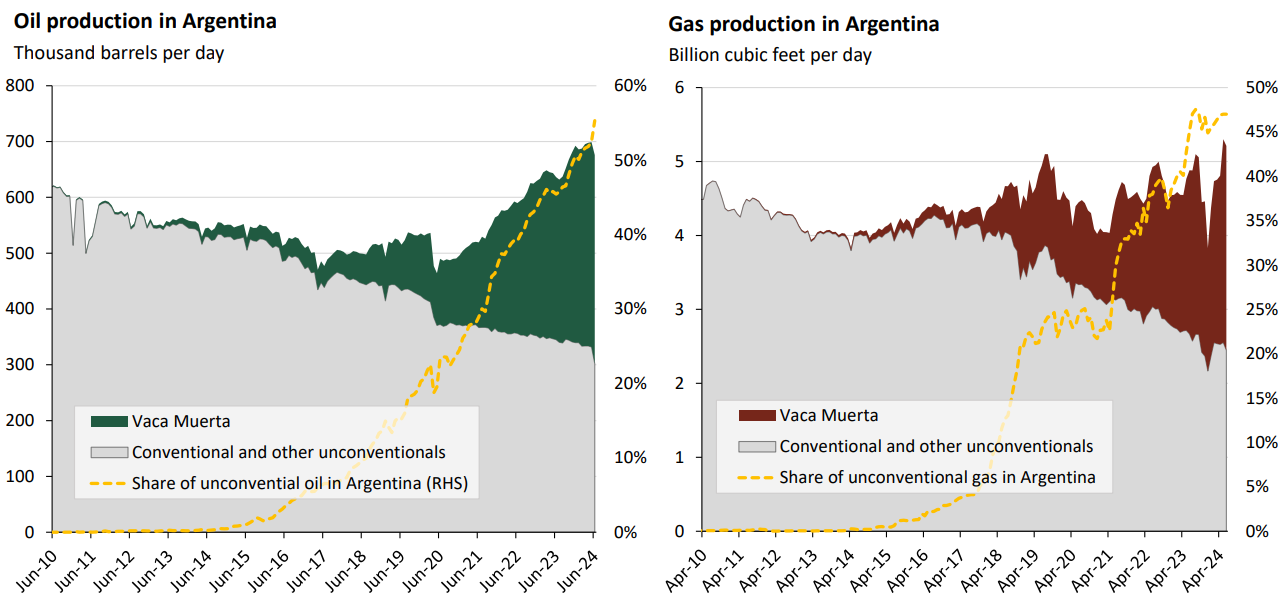
\includegraphics[width=1\linewidth]{figures/ch9/oilgasproduction.png}
    \caption{Oil and gas production in Argentina \autocite{internationaltradeadministrationArgentinaCountryCommercial2025}}
    \label{fig:oilgasprod}
\end{figure}

The numbers in figure \ref{fig:oilgasprod} help explain why fracking in the Neuquén basin is viewed by some as crucial to the development of Argentina's economy. It also becomes clear that, considering the volumes present in the reserves, even more gas and oil could still be extracted.

\subsection{Theoretical background: fracking}
In the 1970's, geologists became increasingly aware that large volumes of gas existed in low-permeability sandstones. However, conventional methods did not allow for economic extraction of gas from these `tight reservoirs' \autocite{lawGasTightReservoirs1992}. Hydraulic fracturing, or fracking, a method first tested in 1947 and applied on a large scale for the first time in the 1970's, is a modern method used to extract oil and natural gas from these low-permeability rock formations, such as shale \autocite{denchakFracking1012019}.

The technique begins by drilling a long vertical well. As soon as the desired rock formation is reached, drilling gradually turns horizontal and steel pipes called `casings' are inserted into the well. Small holes are perforated in the casing and then fracking fluid is pumped in at a pressure high enough to create new fractures or open existing ones in the surrounding rock. This allows previously unavailable oil or gas to flow to the surface \autocite{denchakFracking1012019}.

The fracking fluid contains as much as 97 percent water, but also always contains proppants. These are small, solid particles that keep the fractures in the rock formation open after the pressure from injection is removed. Sand, or more specifically silica sand, is the most widely-used proppant in the fracking industry \autocite{denchakFracking1012019}. 

\subsection{Fracking sand}
Sand is thus an essential substance to keep the drilled pores open and to allow for the fossil fuels to flow out. This sand is mined or imported. In figure \ref{fig:sanddiagram}, the mined silica sand masses as well as the imported masses are given for Argentina.

\begin{figure}[H]
    \centering
    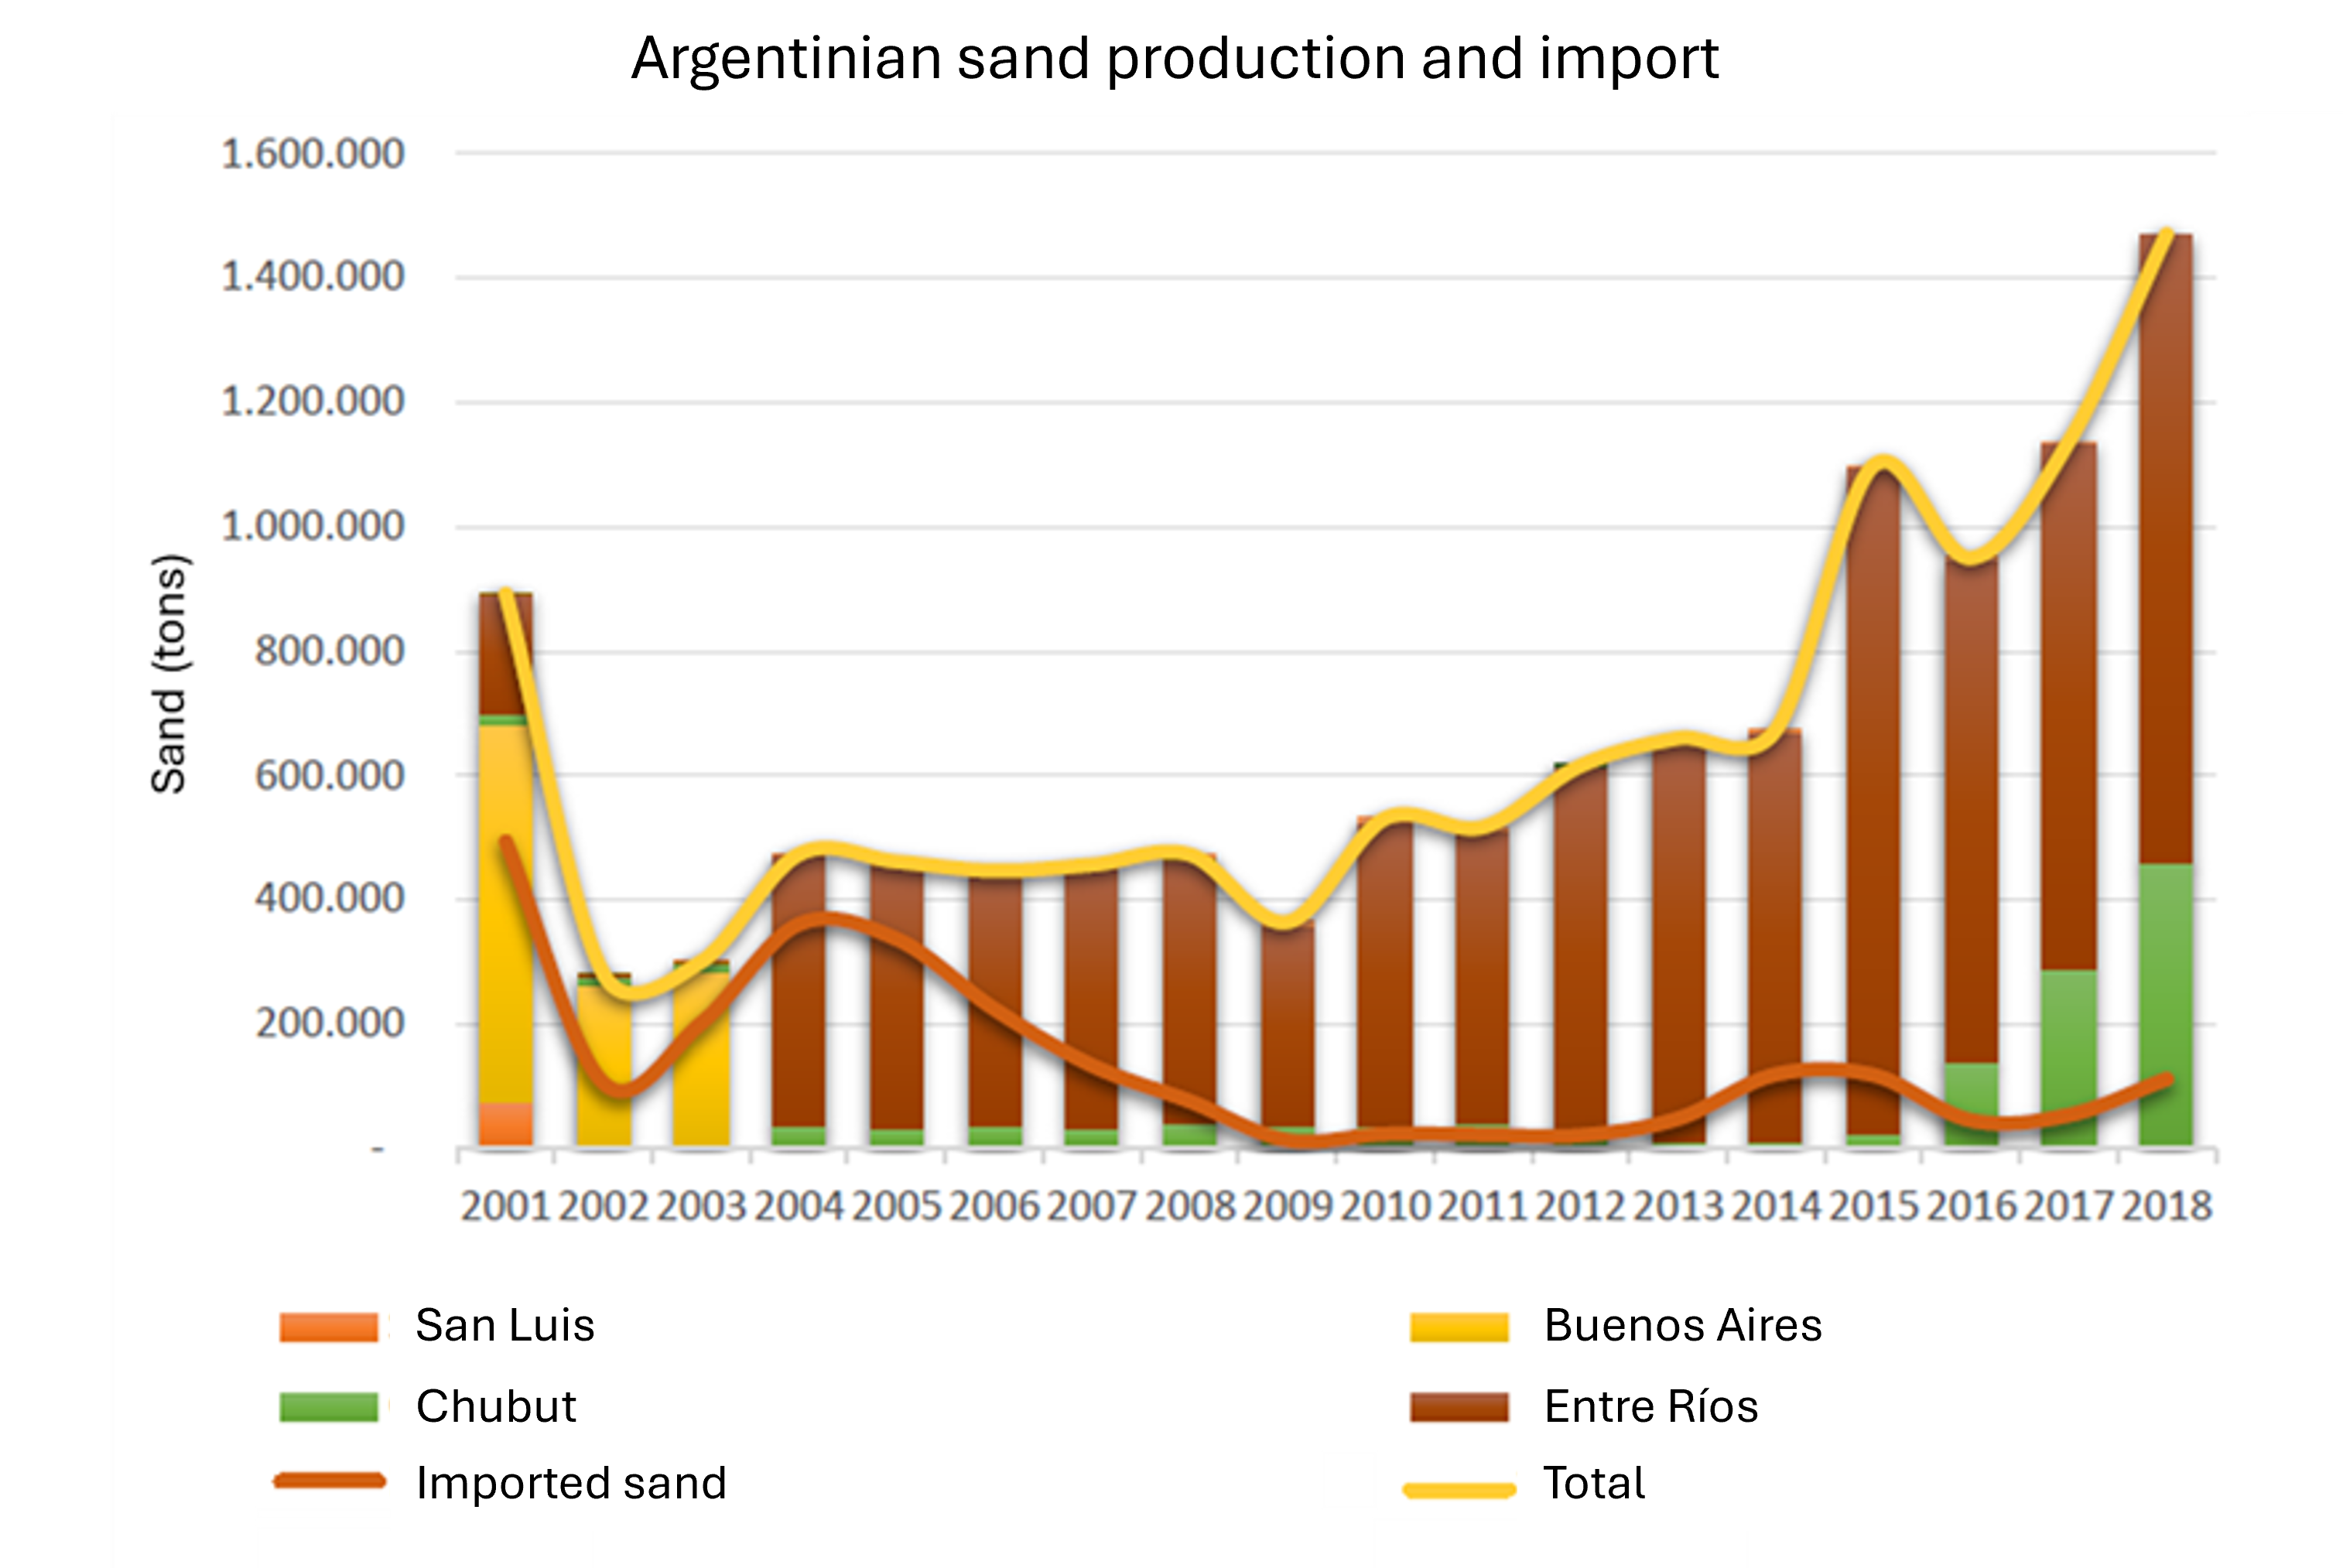
\includegraphics[width=1\linewidth]{figures/ch9/Sandgraphquantities.png}
    \caption{Quantities of sand mined in Argentine provinces, adapted from \cite{secretariadepoliticamineraArenasParaFracking2019}}
    \label{fig:sanddiagram}
\end{figure}

In 2018, 

2018: more than 90\% of used sand from national origin, the rest imported
Percentage Entre Ríos
De totale export van siliciumzand en kwartszand vertegenwoordigt minder dan 1% van de import van dezelfde aggregaten in 2018. De bestemmingen zijn buurlanden: Paraguay, Uruguay, Bolivia en Chili, en in alle gevallen wordt voor transport per vrachtwagen gekozen.
Aantonen dat het voor fracking is? -> Niet bekend maar tegelijk met opmars fracking en ook in rapport

Siliciumzand werd van oudsher beschouwd als een industrieel mineraal dat als grondstof werd gebruikt in de
glasindustrie, waarvan de specificaties bepaalde eigenschappen
vereisten.
De inventarisatie van de afzettingen was dus afhankelijk van de vraag of het zand aan de voorwaarden voldeed
nodig waren voor deze productieve sector. De opkomst van de vraag naar het gebruik ervan in de olie-industrie
verruimde de horizon van de toepassingen van siliciumzand.
Het is niet mogelijk om te weten welk deel van de productie bestemd is voor de exploitatie van niet-conventionele olie.
en welk deel voor meer traditionele toepassingen wordt gebruikt,

Hoewel de vraag naar siliciumzand verspreid is over verschillende industrieën, is de drijvende kracht achter deze vraag de
exploitatie van onconventionele olie. Verwacht wordt dat deze trend zich zal doorzetten, niet alleen vanwege de eisen van
het project in Neuquén, maar ook vanwege andere soortgelijke projecten die zich nog in de exploratiefase bevinden


Van alle departementen waar het bedrijf actief is, is Ibicuy de plaats waar de "boom
van Vaca Muerta" het meest voelbaar is. Bronnen die voor dit artikel zijn geraadpleegd,
schatten dat er dagelijks 350 vrachtwagens uit dit gebied in het zuiden van Entre Ríos
vertrekken. De gemeente zelf voorspelde dat er in 2022 meer dan 1.250.000 ton zand naar
het stroomgebied van Neuquén zou worden vervoerd. Dit is meer dan de totale nationale
winning in 2018.

In Ibicuy zijn onder andere Cristamine, Aresil S. A., YPF, La Chola II, NRG Argentina,
San Marcos Trading en QSand actief. De eerste vier hebben wasinstallaties. Oorspronkelijk
leverden sommige van hen alleen aan de keramiek- en glasindustrie. Tegenwoordig leveren
bedrijven als Aresil hun volledige productie aan de oliesector. La Chola II, met een halve eeuw
ervaring in de winning van riviersand, sloot zich in 2016 aan bij het Vaca Muerta-circuit. Met de
steengroeve Silicatos Islas del Ibicuy en een modulaire fabriek met Ierse technologie die "in
slechts zes dagen" werd geïnstalleerd, wint, wast, sorteert en verzendt het zand voor YPF, zijn
belangrijkste klant(22) .

Maar niet alleen nationale bedrijven hebben belangen in de steengroeven van Entre Ríos. De Belgische Jan de Nul Group, gespecialiseerd in haven- en maritieme engineering, richtte in 2016 Arenas Argentinas del Paraná
op. Volgens eigen zeggen exploiteert het sinds 2019 een steengroeve aan de oever van de rivier El Salto in Diamante, drie kilometer van de plaats Aldea Brasilera en dertig kilometer ten zuiden van de stad Paraná. Daar wint het bedrijf zand met een zuiverheid van bijna 100 %, dat vervolgens in zijn fabriek in dezelfde plaats wordt verwerkt en aan klanten zoals Tecpetrol wordt verkocht.




Hoewel de vraag naar siliciumzand verspreid is over verschillende industrieën, is de drijvende kracht achter deze vraag de exploitatie van onconventionele olie. Verwacht wordt dat deze trend zich zal doorzetten, niet alleen vanwege de eisen van het project in Neuquén, maar ook vanwege andere soortgelijke projecten die zich nog in de exploratiefase bevinden

Transport:
Weg
Weg + spoor

Het nationale zand dat in Vaca Muerta wordt gebruikt, wordt momenteel vervoerd door vrachtwagens die minstens 1300 km afleggen vanuit Entre Ríos. De steengroeven liggen ver van de vindplaatsen. Wegtransport maakt overslag overbodig en bovendien rijdt de vrachtwagen sneller dan de andere vervoersmiddelen. De vrachtwagen doet er ongeveer 20 uur over om het zand bij de put af te leveren , waarbij rekening wordt gehouden met 2 uur vertraging voor het laden en lossen van de goederen. Dagelijks vertrekken er tussen de 70 en 100 vrachtwagens uit Ibicuy, meestal met aanhangwagens die een maximumlading vervoeren van 28 ton zand. Ze beginnen hun reis op de RP 45 Entre Ríos vanaf de toegang tot Ibicuy, een relatief nieuwe weg, maar die te lijden heeft onder het feit dat het een van de meest gebruikte wegen in het zuiden van Entre Ríos is. Van daaruit nemen ze de RN 5 (bij voorkeur) of 3 om Buenos Aires te doorkruisen. Vanaf Diamante kunnen ze de RN 33 nemen. De provincie La Pampa kan worden bereikt via de provincie Buenos Aires, via de RN 188 of RN 5, of de RP 20 of RP 14, of vanuit Córdoba, via de RP 1 of RN 35.

ls u Río Negro binnenkomt via de RN 152, neemt u de RN 232 naar Chacharramendi, op het kruispunt met de RN 22. Andere vrachtwagenchauffeurs kiezen ervoor om de route 20 te nemen om uiteindelijk aan te sluiten op de RN 151, die naar de plaats Contralmirante Cordero leidt. terwijl het gedeelte van de RN 151 tussen de plaats Cruce del Desierto en de brug Punto Unido in dezelfde mate beschadigd is, waardoor auto's, vrachtwagens en bussen ervoor kiezen om over de De RP 20 is een van de wegen die snel in slechte staat raakt berm rijden. Meestal is de bestemming de plaats Añelo, in Neuquén




\subsection{Characteristics of fracking sand}
Sand used in the fracking process must have fairly specific characteristics in order to be usable for fracking. Silicon sand is mainly used for fracking. This is sand with a grain size between 0.0625 and 2.0 millimeters. The quartz grain content must be higher than 90%. 

Means of transport such as waves and currents in rivers promote the removal of finer or organic particles, thereby ensuring a higher percentage of quartz grains. This is one of the reasons why sand from the Paraná Delta is suitable for fracking.
In addition to erosion by water, the action of wind also influences the characteristics of sand. It causes changes in texture and generally makes quartz sand rounder. 

The specifications for silica sand are laid down in the international test standard ISO 13503-2:2006. The important aspects are as follows:

\begin{enumerate}
    \item  Size and distribution of the particles
    \item Shape of the particles
    \item Acid resistance 
    \item Fracture and compressive strength of the grains
    \item Clay and silt content
\end{enumerate}

When it comes to size distributions of the sand particles, the most important is that 90 per cent or more is found in a small size range. Thereby is the size of the particles of less importance and can per badge differ. But when using a sand badge, that badge must have almost exact the same distribution. 

The shape of the sand particles must be round enough and smooth enough to be applicable. Therefore is the system of Krumbrein, W.C. en Sloss, LL. used. This system is shown in \ref{fig:RT}. The norm says that for both roundness as sphericity the value must as least be 0.6. It's important to mention that this procedure is visual and therefore depends on the subjective perception of the person analysing the sample.

\begin{figure}[H]
    \centering
    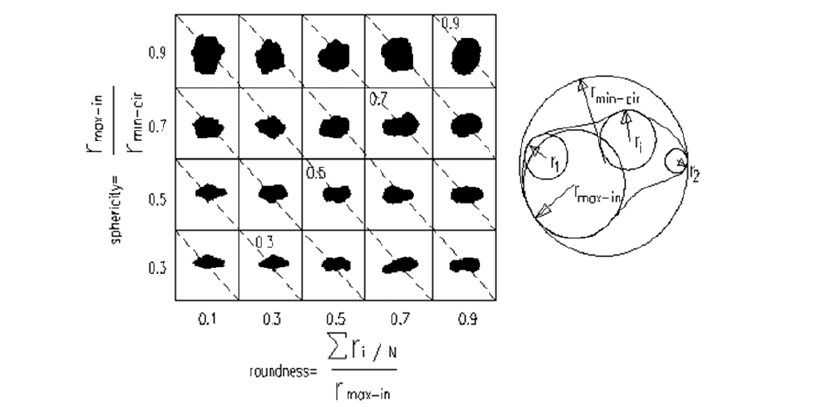
\includegraphics[width=0.75\linewidth]{figures//ch9/roundness.png}
    \caption{Roundness table \autocite{rodriguezParticleShapeQuantities2013}}
    \label{fig:RT}
\end{figure}

Acid solubility testing is used to determine the concentration of soluble elements that contaminate the binder. These elements are typically softer materials that can break down and migrate into the artificially created pore system during fracture closure. This process can lead to conductivity issues within the formation.
To evaluate this are various acids  used of which most are hydrochloric and hydrofluoric acids. These acids dissolve soluble grains such as carbonates, clays, and oxides, while leaving quartz grains intact. Because of this behaviour, industry regulations specify maximum allowable levels of acid-soluble materials that could significantly reduce the permeability of cracks in the wells.
For coarser frac sand with a grain size up to 30/50 mesh, a maximum of 2\% acid-soluble content is permitted. For finer sands, this limit increases to 3\%, as shown in \ref{tab:acid} below.

\begin{table}[h!]
\centering
\begin{tabular}{|c|c|c|}
\hline
\textbf{Particle size (ASTM)} & \textbf{Particle size (mm)} & \textbf{Max. solubility (\% by weight)} \\ \hline
6/12 to 30/50 & 1.68/3.36 to 0.30/0.60 & 2.0 \\ \hline
40/70 to 70/140 & 0.21/0.42 to 0.10/0.21 & 3.0 \\ \hline
\end{tabular}
\caption{\textit{Recommended maximum acid solubility}}
\label{tab:acid}
\end{table}

For the compressive strength of grains is a test conducted which puts a pressure on the sand particles and then sieves the sample to look which percentage of the particles go trough a certain sieve. This percentage of breaking particles in combination with the known applied pressure tells us which pressure the sand can withstand when using it for making cracks.
The permeability of the fracks in the oil sources drops rapidly if the percentages of cracking sand particles and clay/silt particles is too high. 

\subsubsection{characteristics of Ibicuy specific}

The sand of the Ibicuy region in the province of the Entre Rios is mostly composed of quarts (86\%). But the sand is quite polluted by iron minerals. The percentage of heavy minerals is very low (0.3\%). This is one of the reasons that the sand is washed before transporting it to the fracking plants. 

\subsection{Consequences of dry sand mining}

\subsection{Recommendations and mitigation strategies}

\subsection{Geological conditions}
To understand more about the region and in order to be able to design mitigation measures in a later stage, the characteristics of the regional subsoil were researched. This section intends to combine all the available information regarding the subsoil in the investigation area.

\subsubsection{The geology of a delta}
A delta is a landscape formed at the mouth of a river where the water eventually runs into the ocean. At a delta, the water's velocity decreases which gives floating particles in the delta the change to settle. Among these floating particles are gravels, sands and clays, descending in particle size. The particles are formed by erosion of stone. The origin of the particles in the Parana river are the Andes mountains. 
Besides that, deltas are also characterized by high vegetation growth. When this vegetation dies, the organic material will change into peat due to the governing pressures. So, in a delta one expects to find relatively soft soils (sands) and very soft soils (clay and peat).

\subsubsection{Geological cross sections}
A study by \citeauthor{joseluiscavallottoEvolucionCambiosAmbientales2005} was conducted that led to a morphological map of the Paraná delta. In the study, for two cross sections a more detailed geological profile was made, one of which is relevant to the area of interest. The cross section along with the area of interest is shown in figure \ref{fig:crosssectiongeo}.

\begin{figure}[H]
    \centering
    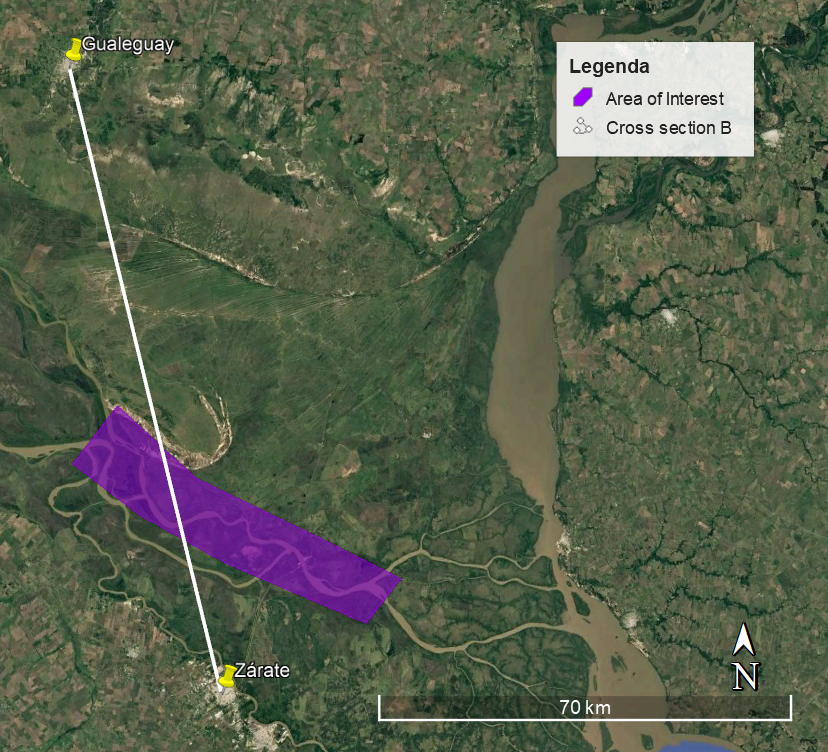
\includegraphics[width=0.75\linewidth]{figures/ch9/CrossSectionB.png}
    \caption{Cross section}
    \label{fig:crosssectiongeo}
\end{figure}

The geological profile of the cross section is shown in figure \ref{fig:geolprofile}. As can be seen in the figure, the taken cross section was around 80 km long. Of this, 15 km falls inside the area of interest, this zone is marked with purple.

\begin{figure}[H]
    \centering
    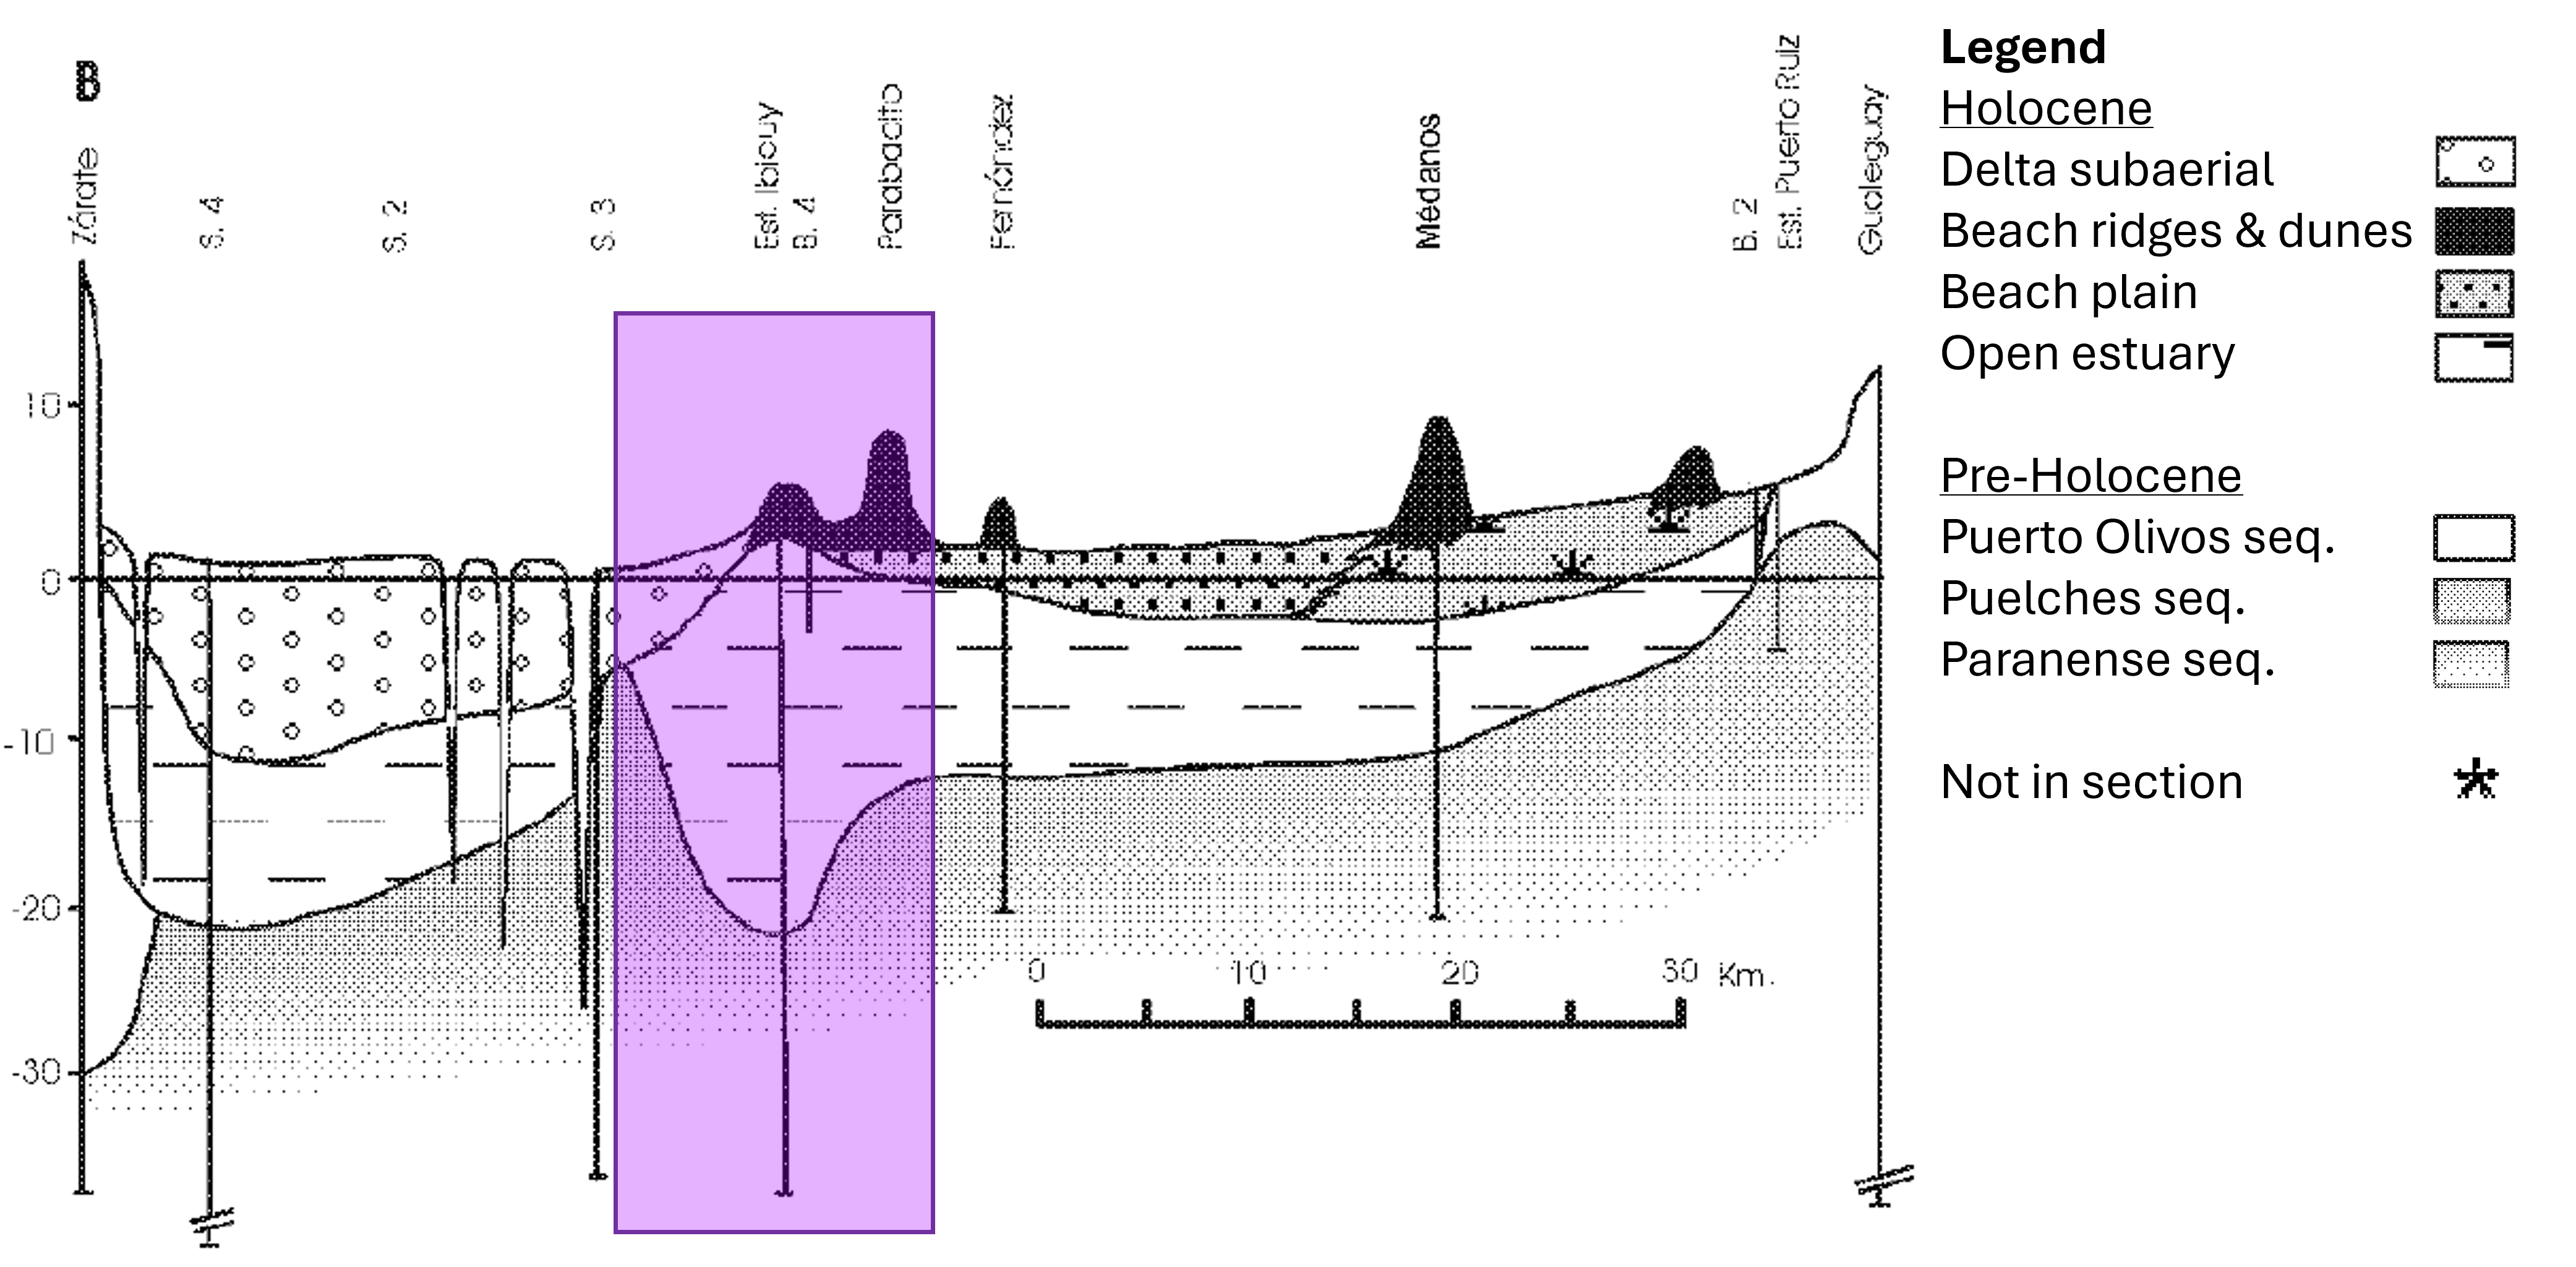
\includegraphics[width=1\linewidth]{figures/ch9/CrossSectionBResults.png}
    \caption{Geological profile of cross section \autocite{joseluiscavallottoEvolucionCambiosAmbientales2005}}
    \label{fig:geolprofile}
\end{figure}

In figure \ref{fig:geolprofile}, the first kilometers of the purple zone are especially of interest since these are located near the river. The following layers can be identified in this area.

The subaerial facies of the Paraná Delta developed through the deposition of silty-sandy sediments delivered mainly by the Paraná Guazú and Paraná de las Palmas \autocite{joseluiscavallottoEvolucionCambiosAmbientales2005}. These deposits occur at elevations between 2 m and sea level, with a maximum thickness of 12 m. This is the layer that is drained.

Mineralogical analyses show a predominance of quartz with minor plagioclase and K-feldspar, plus heavy minerals such as magnetite, hematite, garnet, zircon, tourmaline, and others, generally well-rounded except zircon, which preserves crystal form \autocite{rafaelcordiniContribucionConocimientoGeologia1949}. The age of the unit is debated: radiocarbon dates suggest origin dates between -150 BC and 180 AD, while other authors propose a later origin around 700–750 AD \autocite{joseluiscavallottoEvolucionCambiosAmbientales2005}.

The open estuary sediments were deposited during postglacial sea-level rise and were formed at the freshwater–saltwater interface during the upstream migration of the maximum salinity gradient, which filled the Río de la Plata river valley \autocite{joseluiscavallottoEvolucionCambiosAmbientales2005}.

These are olive-green clays to silty clays with thin fine-sand layers, scattered or concentrated shell beds, and fossil content confirming estuarine conditions. The unit is dated to the Holocene, with its base at ~6670 +/- 100 years BC, occurring between –22 and –0 m and reaching up to 20 m thick \autocite{vogelGroningenRadiocarbonDates1969}.

During the Miocene, large portions of present-day Argentina, Uruguay, Paraguay, southern Brazil, and eastern Bolivia were covered by the Paranense Sea. This was a shallow sea that advanced from the Atlantic into the interior of South America . Its waters left behind extensive marine sediments and fossils and this layer is now known as the Paranense depositional sequence \autocite{tineoReconstructingSouthAmerican2024}.

It is composed mainly of siliciclastic sandstones, mudstones, and bioclastic beds, with thicknesses ranging from a few meters in outcrop to over 100 m. The lower part has mud-dominated offshore deposits with marine fossils, while the upper part shows sandier shoreface. Studies constrain the unit to the Late Miocene (ca. 9.5–6.7 Ma) \autocite{tineoReconstructingSouthAmerican2024}.

Another study focuses on subsurface deposits from Diamante in Entre Ríos to San Fernando in the Buenos Aires province. Based on lithologic, clay mineral, radiocarbon, and outcrop data, the authors propose a depositional model for the region. This geological cross section is shown in figure \ref{fig:depmodel}. The purple area marks the area of interest for this research (Puerto Ibicuy).

\begin{figure}[H]
    \centering
    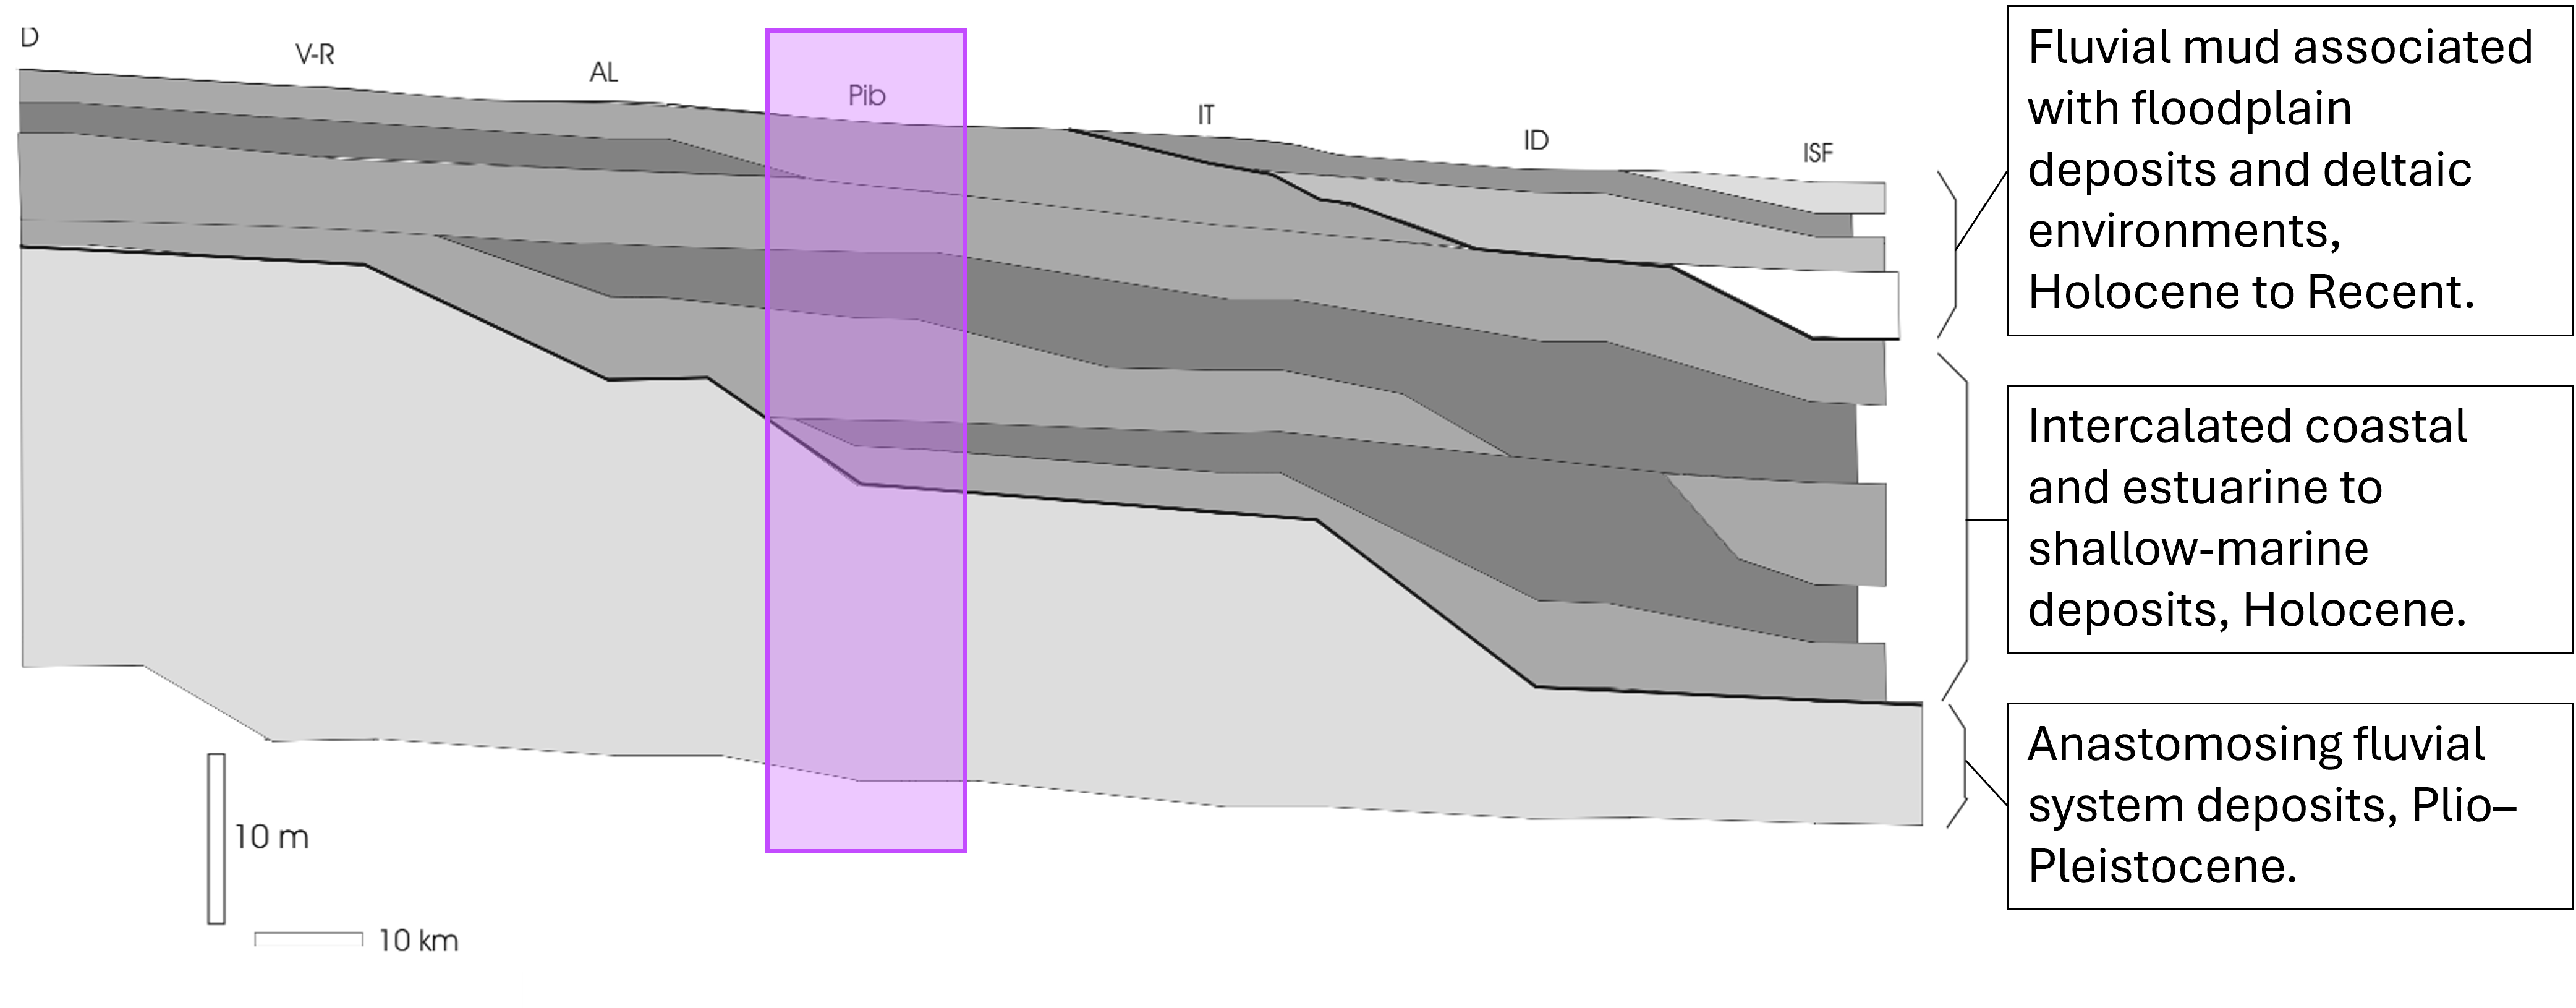
\includegraphics[width=1\linewidth]{figures/ch9/Crosssection2.png}
    \caption{Depositional model \autocite{amatoESTRATIGRAFIACUATERNARIASUBSUELO2009}}
    \label{fig:depmodel}
\end{figure}

As can be seen in the figure, the first layer consists of deltaic and flooplain deposits from the Holocene until recent times. This is in accordance with the geological profile as shown in figure \ref{fig:crosssectiongeo}. Underneath, holocene coastal/estuarine sediments can be found and below there are the Plio–Pleistocene fluvial deposits. The estuarine sediments can also be found in figure \ref{fig:crosssectiongeo}, but a different conclusion was reached for the final layer. \citeauthor{joseluiscavallottoEvolucionCambiosAmbientales2005} conclude that this is a pre-holocene marine deposit from the Miocene Paranense Sea, while here Plio–Pleistocene river deposits are placed below the Holocene sequence.

\subsection{Borehole}
In the same study conducted by \citeauthor{amatoESTRATIGRAFIACUATERNARIASUBSUELO2009}, a number of boreholes were executed along the lower Paraná \autocite{amatoESTRATIGRAFIACUATERNARIASUBSUELO2009}. One of these boreholes were executed near the area of interest in Puerto Ibicuy. The borehole was interpreted and with this the following soil profile was made  \autocite{amatoESTRATIGRAFIACUATERNARIASUBSUELO2009}.

\begin{figure}[H]
    \centering
    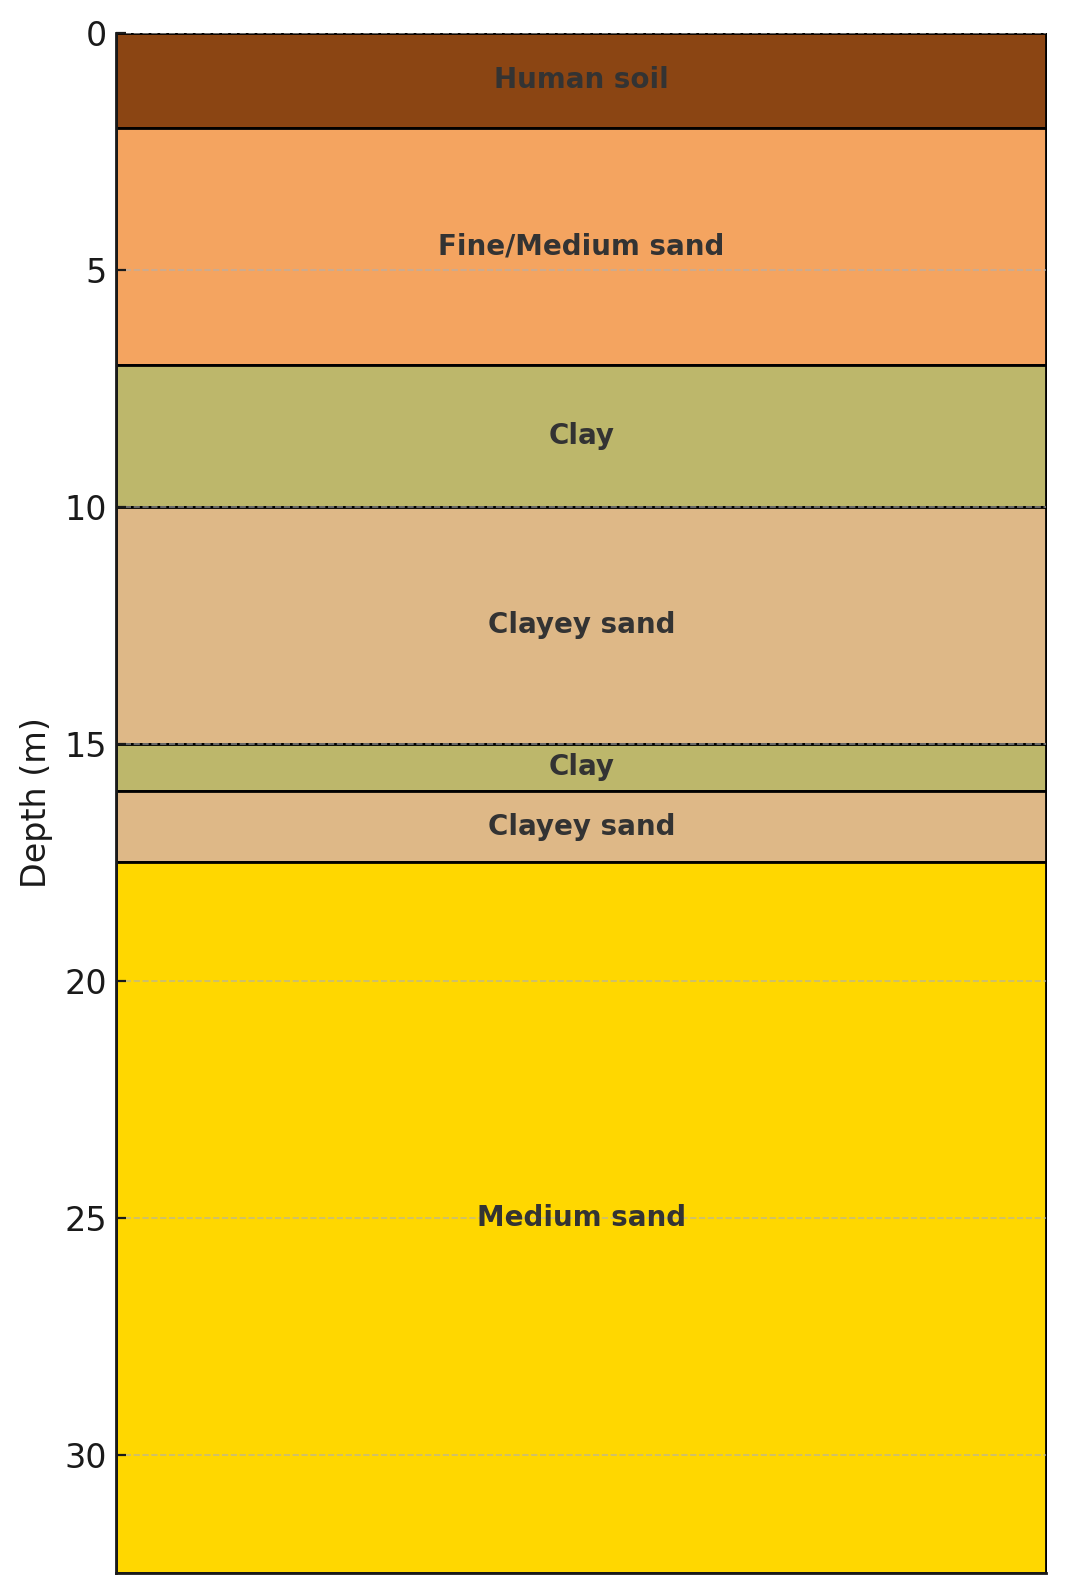
\includegraphics[width=0.45\linewidth]{figures//ch9/Bodemprofiel.png}
    \caption{Borehole profile in Puerto Ibicuy \autocite{amatoESTRATIGRAFIACUATERNARIASUBSUELO2009}}
    \label{fig:borehole}
\end{figure}

\subsection{Geotechnical summary}
To be able to design mitigation measures, the soil layers along with their geotechnical parameters should be known. For this, the borehole is deemed the most relevant source. The borehole shows a top layer with fine/medium sands. Below, clay/clayey sand can be found, and the bottom layer consists of medium sand. This is in accordance with the geological profiles that were provided before in figures \ref{fig:crosssectiongeo} and \ref{fig:depmodel}. Both frameworks describe a fluvial-to-estuarine-to-marine vertical transition. The top fluvial deposits help declare the presence of sandy deposits at the top and the layers of clay/clayey sand below correspond to estuarine deposits. Finally, old marine/fluvial deposits were likely compacted and lead to the layer of medium sand found at the bottom of the borehole.

Because of the resemblance between the local borehole and geological profiles given before, the layering as shown in figure \ref{fig:borehole} is deemed representative for the whole study area. Based on this layering the relevant parameters can be derived, the result in shown in table \ref{tab:soil_layers}.

\begin{table}[H]
    \centering
    \begin{tabular}{|c|c|c|c|c|c|c|c|}
        \hline
        Start layer (m) & End layer (m) & Soil type & \makecell{ $\gamma_d$ \\ (kN/m$^3$) } & \makecell{ $\gamma_{sat}$ \\ (kN/m$^3$) } & \makecell{ $\varphi'$ \\ ($^\circ$) } & \makecell{ $c'$ \\ (kPa) } & \makecell{ $c_u$ \\ (kPa) } \\
        \hline
        0 & 2 & Fill (Topsoil/Agricultural) & 12 & 12 & 15 & 2.5 & 20 \\
        2 & 7 & Fine/medium sand & 17 & 19 & 30 & 0 & - \\
        7 & 10 & Clay & 14 & 14 & 17.5 & 0 & 25 \\
        10 & 15 & Clayey sand & 18 & 20 & 25 & 0 & - \\
        15 & 16 & Clay & 14 & 14 & 17.5 & 0 & 25 \\
        16 & 17.5 & Clayey sand & 18 & 20 & 25 & 0 & - \\
        17.5 & 32 & Medium sand & 18 & 20 & 32.5 & 0 & - \\
        \hline
    \end{tabular}
    \caption{Soil stratigraphy and geotechnical properties.}
    \label{tab:soil_layers}
\end{table}

The parameters in table \ref{tab:soil_layers} were derived from the Eurocode \autocite{stichtingkoninklijknederlandsnormalisatieinstituutNederlandseNormNEN2025}. Because of limited knowledge on soil characteristics, conservatives estimates were made based on this code. In the borehole, no explicit information is given on the top fill layer. Therefore, conservative parameters are assumed based on typical values for organic topsoil.